\subsubsection{文字列のパッチ(Win32)}

Hiewを使用して、実行可能ファイル内の ``hello、world'' 文字列を簡単に見つけることができます:

\begin{figure}[H]
\centering
\myincludegraphics{patterns/01_helloworld/hola_edit1.png}
\caption{Hiew}
\label{}
\end{figure}

メッセージをスペイン語に翻訳しようとすることができます

\begin{figure}[H]
\centering
\myincludegraphics{patterns/01_helloworld/hola_edit2.png}
\caption{Hiew}
\label{}
\end{figure}

スペイン語のテキストは英語より1バイト短くなっているので、最後に0x0Aバイト(\TT{\textbackslash{}n})に続けてNULLバイトを追加しました。

うまくいきました。

より長いメッセージを挿入する場合はどうすればよいですか?
元の英語テキストの後には、ゼロバイトがいくつかあります。 上書きできるかどうかはなんとも言えません:\ac{CRT}コードのどこかで使われるかもしれないし、そうでないかもしれません。 
とにかく、自分が行っていることを本当に知っていれば、それらを上書きするだけです。

\subsubsection{文字列のパッチ(Linux x64)}

\myindex{\radare}
\radare{}を使ってLinux x64実行ファイルにパッチを当ててみましょう

\lstinputlisting[caption=\radare{} session]{patterns/01_helloworld/radare.lst}

ここでは何が起こっているの:私は\TT{/}コマンドを使用して\q{hello}文字列を検索し、
そのアドレスに\emph{カーソル}(\radare{}用語で\emph{シーク})を設定します。 
次に、これが本当にその場所であることを確かめたい:\TT{px}がダンプします。
\TT{oo+}は\radare{}を\emph{読み書き}モードに切り替えます。 
\TT{w}は現在の\emph{シーク}時にASCII文字列を書き込みます。
最後の\TT{\textbackslash{}00}に注意してください。これはNULLバイトです。
\TT{q}で終了します。

% TBT
%\subsubsection{This is a real story of software cracking}
%\label{\SoftwareCracking}
%
%An image processing software, when not registered, added watermarks,
%like ``This image was processed by evaluation version of [software name]'', across a picture.
%We tried at random: we found that string in the executable file and put spaces instead of it.
%Watermarks disappeared.
%Technically speaking, they continued to appear.
%\myindex{Qt}
%With the help of Qt functions, the watermark was still added to the resulting image.
%But adding spaces didn't alter the image itself...

\subsubsection{MS-DOS時代におけるソフトウェアの\emph{ローカライズ}}

このやり方は、1980年代と1990年代にMS-DOSソフトウェアをロシア語に翻訳する一般的な方法でした。 ロシア語の言葉や文章は、英語の文章と比べて通常若干長いので、\emph{ローカライズ}されたソフトウェアには奇妙な頭字語やとても読みにくい略語が含まれています。

\begin{figure}[H]
\centering
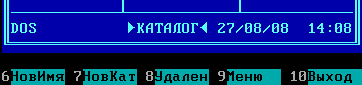
\includegraphics[width=0.5\textwidth]{patterns/01_helloworld/Norton_Commander_v5_51.png}
\caption{\JPph{}}
\end{figure}

他の国の他の言語でも、この時代に起きていたことでしょう。
